\section{Introduction} % A complete overview

% DONE Introduces the larger reasearch area that the paper is part of
% DONE Illustrates the concrete problem
% Explains the proposed solution
% Highlights the main results
% Might finish with a short explanation of the following sections

In computer architecture, the ``memory wall''~\cite{wulf_mckee_1995}
is a well known problem. Slow memory act as a bottleneck in a system
with fast processors. The reason for this is that processors will
request data faster than what primary memory can provide. In a Von
Neumann architecture~\cite{von1992first}, the processor
will stall as it waits for the next data or instruction to arrive.

\begin{center}
  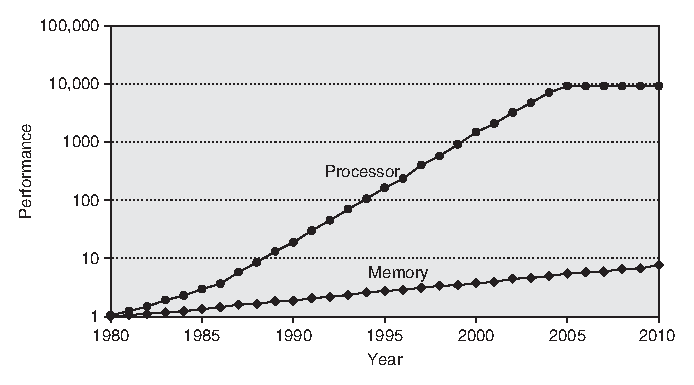
\includegraphics[width=0.5\textwidth]{graphs/memorywall}
  \captionof{figure}{The Memory Wall}
\end{center}

There are several techniques used in modern systems which mitigates
this bottleneck, like caching or outsourcing memory management to a
DMA. One interesting approach is named ``prefetching''.

Prefetching involves speculating in which memory addresses are needed
in the near future, and fetching them prior to execution. This paper
investigates the ``speculating'' part, that is, what addresses should
be fetched and when. When the prefetching is successful, CPU stalling
is avoided as the processor has the needed data available, resulting
in increased performance. When unsuccessful, valuable cache space is
wasted.

The most basic kind of prefetching would be to load the memory
addresses which sequentially follow the address we are currently
working on. However, this tends to be not so effective as memory
access tend to be non-sequential. Instead, we can look for access
patterns, and try to exploit them.

In this paper we start by exploring the sequential prefetcher. A
Stride Directed Prediction prefetcher, a slight improvement to the
previous. Later
we implement both a Global Histor Buffer and Reference Prediction
Table prefetcher with a speedup compared to baseline of 3\%. 


% http://ieeexplore.ieee.org/abstract/document/5389383/
